\documentclass[10pt]{beamer}

% \usepackage[table,xcdraw]{xcolor}
\usepackage[square,numbers]{natbib}
\usepackage{graphicx}
\usepackage{svg}
\usepackage{pgfplots}
\usepgfplotslibrary{dateplot}

% \usetheme[progressbar=frametitle]{metropolis}
\usecolortheme{Imperial}
\usepackage{appendixnumberbeamer}

\usepackage{booktabs}
\usepackage[scale=2]{ccicons}


\usepackage{pgfplots}
\usepgfplotslibrary{dateplot}
\usepackage{xspace}
\newcommand{\themename}{\textbf{\textsc{metropolis}}\xspace}

\usepackage{amsfonts, amsmath, amsthm, amssymb}
\usepackage{bbm}
\usepackage{bm}
\usepackage{mathtools}
\usepackage[ruled,vlined]{algorithm2e}
\newlength{\commentWidth}
\setlength{\commentWidth}{7cm}
\newcommand{\atcp}[1]{\tcp*[r]{\makebox[\commentWidth]{#1\hfill}}}
\usepackage{setspace}
\usepackage[utf8]{inputenc}

\newcommand*{\QEDA}{\hfill\ensuremath{\blacksquare}}%
\newcommand*{\QEDB}{\hfill\ensuremath{\square}}%

\usepackage{tikz}
\usepackage{tikz-qtree}
\usepackage{forest}
\usetikzlibrary{trees} % this is to allow the fork right path

\setbeamertemplate{itemize items}[circle]
\setbeamertemplate{enumerate items}[default]
\usefonttheme[onlymath]{serif}


\title{\textbf{EDPs via Fluxo de Gradiente em \\Espaços de Wasserstein}}
\subtitle{}
% \date{\today}
\date{}
\author{\textbf{Autor:} Davi Sales Barreira \\\hfill\\}
\institute{
\includegraphics[height=0.55cm]{emaplogo.png}}
\titlegraphic{
\includegraphics[height=0.35cm]{emaplogo-neg.png}}


\usepackage{caption}
\captionsetup[figure]{font=footnotesize}

\begin{document}

\maketitle

\begin{frame}{Sumário}
  \setbeamertemplate{section in toc}[sections numbered]
	\setbeamertemplate{subsection in toc}[subsections numbered]
	% \setbeamerfont{section in toc}{size=\normal}
	\setbeamerfont{subsection in toc}{size=\small}
  % \tableofcontents[hideallsubsections]
  \tableofcontents[sectionstyle=show, subsectionstyle=show]
\end{frame}

\AtBeginSection{}
\section[Ideia Geral]{Ideia Geral e Motivação}
\begin{frame}[fragile]{Ideia Geral}

O espaço de Wasserstein se trata de um espaço métrico de medidas
de probabilidade embutido com a métrica de Wasserstein.
\vspace{3mm}

Um Fluxo de Gradiente é um sistema de equações onde a evolução do sistema se
dá através da descida de gradiente.
\vspace{3mm}

A ideia geral dessa apresentação é mostrar como algumas EDPs
podem ser reformuladas em termos de um Fluxo de Gradiente
em um espaço de Wasserstein. Apresentaremos como reformular a equação de calor, porém,
esse método é mais geral, sendo aplicável para muitas outras EDPs.

\end{frame}

\begin{frame}[fragile]{Motivação}

Por que interpretar EDPs como Fluxo de Gradiente em Wasserstein?
\vspace{3mm}
\begin{enumerate}
	\item Estética. Veremos que é uma bela interpretação que permite
	entender as EDPs de outro ponto de vista;
	\item Reformulação permite utilizar outros ferramentais
	para demonstrar, por exemplo, taxas de convergência,
	existência e unicidade;
	\item Esquema de discretização de fluxos de gradiente
	como algoritmo para aproximar soluções fracas
	para as EDPs.
\end{enumerate}

\end{frame}

\AtBeginSection{}
\section[Teoria de Transporte Ótimo]{Teoria de Transporte Ótimo}
\subsection[Teoria OT]{Monge \& Kantorovich}
\begin{frame}[fragile]{Teoria OT - Monge \& Kantorovich}

\textbf{Problema de Monge} -
Qual a maneira ótima de transporta massa de uma configuração
para outra?
\vspace{3mm}

\begin{figure}[H]
  \centering
  \def\svgscale{0.4}
  \includesvg[inkscapelatex=false]{Figures/mongeproblem.svg}
  \caption{Massa não pode ser separada.}
  \label{fig:mongeproblem}
\end{figure}

\textbf{Kantorovich Problem} -
Relaxação do problema original de Monge.
\vspace{3mm}

\begin{figure}[H]
  \centering
  \def\svgscale{0.4}
  \includesvg[inkscapelatex=false]{Figures/kantorovichproblem.svg}
  \caption{Massa pode ser separada.}
  \label{fig:kantorovichproblem}
\end{figure}

\end{frame}


\begin{frame}[fragile]{Teoria OT - Monge \& Kantorovich}
	
\begin{definition}[Problema de Monge]
	Dadas duas medidas de probabilidade $\mu \in \mathcal P(X)$,
  $\nu \in \mathcal{P}(Y)$ e uma função de custo
  $c:X\times Y \to[0,+\infty]$, resolva:
  \begin{flalign}
    (MP) &&
    \inf
    \left\{
    \int_{X} c(x,T(x))d\mu \quad : \quad
    T_\# \mu = \nu
    \right\}&&
  \end{flalign}

\end{definition}

\begin{figure}[H]
  \centering
  \def\svgscale{0.45}
  \includesvg[inkscapelatex=false]{Figures/monge_map_example.svg}
  \caption{Exemplo de dois problemas de Transporte Ótimo.}
  \label{fig:monge_map_example}
\end{figure}
	 
\end{frame}

\begin{frame}[fragile]{Teoria OT - Monge \& Kantorovich}

\begin{definition}[Acoplamento]
	Sejam $(X,\mu)$ e $(Y,\nu)$ espaços de probabilidade. Para
  $\gamma \in \mathcal{P}(X\times Y)$, dizemos que $\gamma$
  é um acoplamento de $(\mu,\nu)$ se $(\pi_X)_\# \gamma = \mu$
  e $(\pi_Y)_\# \gamma = \nu$. Chamamos $\Pi(\mu,\nu)$
  do conjunto de \textbf{Planos de Transporte}:
  \begin{equation}
    \Pi(\mu,\nu) :=
    \left \{
    \gamma \in \mathcal{P}(X \times Y) \ :
    \ (\pi_X)_\# \gamma = \mu \quad
    \text{and} \quad
    (\pi_Y)_\# \gamma = \nu
    \right \}
  \end{equation}
\end{definition}

	
\begin{definition}[Problema de Kantorovich]
  Dadas duas medidas de probabilidade $\mu \in \mathcal P(X)$,
  $\nu \in \mathcal{P}(Y)$ e a função de custo
  $c:X\times Y \to[0,+\infty]$, resolva:
  \begin{flalign}
    (KP) &&
    \inf
    \left\{
    \int_{X \times Y} c(x,y)d\gamma \ : \
    \gamma \in \Pi(\mu,\nu)
    \right\}&&
    \label{eq:KP2}
  \end{flalign}
  \label{def:KP}
\end{definition}

\end{frame}

\begin{frame}[fragile]{Teoria OT - Problema Dual}

	O Problema de Kantorovich tem uma formulação dual, que
	para certas condições de regularidade possui a mesma
	solução ótima que o problema primal (dualidade forte).

\begin{definition}[Problema Dual]
  Dadas $\mu \in \mathcal P(X)$, $\nu \in \mathcal P (Y)$ e
  custo $c:X \times Y \to \mathbb R_+$. O
  Problema Dual é
\begin{flalign}
  \mathrm{(DP)} &&
  \sup \left \{
  \int_X \phi \ d\mu + \int_Y \psi \ d\nu \ :
  \phi \in C_b(X) \ , \psi \in C_b(Y) \ ,
  \ \phi \oplus \psi \leq c
  \right \}
  &&
  \label{eqt:dualproblem}
\end{flalign}
\end{definition}

Funções $\phi, \psi$ são chamdas de \textbf{Potenciais de Kantorovich}.

\end{frame}

\subsection{Distância de Wasserstein}
\begin{frame}[fragile]{Teoria OT - Distância de Wasserstein}

\begin{definition}[Distância de Wasserstein]

  Seja $(X,d)$ um espaço métrico polonês, com $c:X \times X \to \mathbb R$ tal que $c(x,y)=d(x,y)^p$, e
  $p \in [1,+\infty)$.
  Para $\mu,\nu \in \mathcal P_p(X)$, a distância de Wasserstein é dada por:
  \begin{equation}
    W_p(\mu,\nu) :=
    \left(
    \inf_{\gamma \in \Pi(\mu,\nu)}
    \int_{X \times X} d(x,y)^p \ d\gamma
    \right)^{1/p}
    \label{def:Wasserstein}
  \end{equation}
\end{definition}

$\mathcal P_p(X)$ é o espaço de medidas de probabilidade com$p$-ésimo momento.

\end{frame}

\begin{frame}[fragile]{Teoria OT - Distância de Wasserstein}

	É possível mostrar que a distância de Wasserstein $W_p$ é de fato uma métrica
	no espaço de probabilidade $\mathcal P_p(\Omega)$.

	Além disso, ela metriza a convergência fraca de medidas de probabilidade,
	i.e., sejam $\mu_n, \mu \in \mathcal P_p(\mathbb R^n)$, então
	\begin{equation}
		\mu_n \rightharpoonup \mu \iff W_p(\mu_n, \mu) \to 0.
	\end{equation}

\end{frame}

\subsection{Existência de Soluções}
\begin{frame}[fragile]{Teoria OT - Existência de Soluções}

	Outro aspecto que temos que abordar são as condições de existência das soluções.
	\begin{theorem}[Existência de Planos de Transporte]
		Sejam $X$ e $Y$ espaços métricos poloneses (complete and separável).
		Dados $\mu\in \mathcal{P}(X)$, $\nu \in \mathcal P(Y)$ e
		$c:X\times Y \to[0,+\infty]$, se $c$ for inferiormente semi-continua, então
		(KP) possui solução.
		\label{thm:existanceKPpolish}
	\end{theorem}
	\begin{theorem}[Existência de Mapas de Transporte]
		Seja $\Omega \subset \mathbb R^n$ compacto, e 
		$c(x,y) = h(x-y)$ com $h$ estritamente convexa.
		Dado $\mu \ll \lambda$, e $\partial \Omega$ negligenciável.
		Então, existe solução para o problema de transporte de Monge,
		e além disso
		\begin{equation}
			T(x) = x - (\nabla h)^{-1}(\nabla \phi(x)).
		\end{equation}
		Onde $\phi(x)$ é o potencial de Kantorovich e $T$ é o
		mapa de transporte ótimo.
		\label{thm:existanceMonge}
	\end{theorem}

\end{frame}

\subsection{Formulação Dinâmica}
\begin{frame}[fragile]{Teoria OT - Formulação Dinâmica}

	O problema original de Transporte Ótimo é formulado de forma
	que o transporte ocorre de forma ``instantânea'', porém,
	é possível partir de premissas mais fundamentais, e
	encontrar uma formulação dinâmica para o problema,
	onde a solução não é mais um plano, mas sim uma
	curva $\gamma:[0,1] \to \mathcal P(\Omega)$, com
	$\gamma(0)=\mu$ e $\gamma(1) = \nu$.

\end{frame}

\begin{frame}[fragile]{Teoria OT - Formulação Dinâmica}

	Baseado nessa formulação dinâmica, é possível provar o
	seguinte resultado:

	\begin{theorem}{(Benamou-Brenier Formula)}
	\label{theorem.Benamou-Brenier}
	Sejam $\rho_0, \rho_1 \in \mathcal P_p(\Omega)$ para $p>1$.
	Então, a seguinte caracterização é válida para espaços com a distância p-Wasserstein:
	\begin{equation*}
	\frac{1}{p}W^p_p(\rho_0, \rho_1) 
	= 
	\inf_{(\rho, v)}
	\left\{
	\int_0^1\int_{\Omega}\left|v(t,x)\right|^p d \rho_t(x)d t: \text{Condições B.B}
	\right\}.
	\end{equation*}
	Onde as condições de Benamou-Brenier são
	\begin{align*}
	&(\rho_t)_{t \in [0,1]} \text{ Absolutamente Contínua no espaço de Wasserstein}, \\
	&(\rho_t, v_t)_{t \in [0,1]} \text{é solução fraca de }
	\partial_t \rho_t + \nabla\cdot\left(\rho_t v_t\right) = 0
	\\
	&\rho(0,\cdot) = \rho_0, \ \rho(1, \cdot) = \rho_1 .
	\end{align*}
\end{theorem} 
\end{frame}

\AtBeginSection{}
\section[Fluxo de Gradiente em Wasserstein]{Fluxo de Gradiente em Wasserstein}
\subsection{Introdução ao Fluxo de Gradiente}
\begin{frame}[fragile]{Introdução ao Fluxo de Gradiente}

	Seja uma função $F:\mathbb R^n \to \mathbb R \in C^1$, e $x_0 \in \mathbb R^n$,
	onde queremos descobrir $x(t)$ que resolve o seguinte sistema de equações:
	\begin{equation}
		\begin{cases}
			x'(t) = -\nabla F(x(t)), \ t>0,\\
			x(0)  = x_0.
		\end{cases}
		\label{eq:fluxograd}
	\end{equation}

	A solução $x(t)$ do sistema acima será uma curva iniciando em $x_0$ e se movendo
	na direção de menor gradiente, ou seja, a solução é dada
	pelo famoso algoritmo de descida de gradiente. Em outras palavras,
	a solução $x(t)$ caracteriza um fluxo de gradiente.

\end{frame}

\begin{frame}[fragile]{Introdução ao Fluxo de Gradiente}

	Esse problema é simples quando estamos em espaços de dimensão finita e com
	funções diferenciáveis, porém, torna-se mais
	interessante e complexo quando começamos a considerar espaços de dimensão infinita
	como $\mathcal P_2(\mathbb R^n)$. Neste cenário, temos que repensar, por exemplo,
	a ideia de gradiente, já que não está mais claro que seria o gradiente quando
	$x(t) = \rho_t \in \mathcal P_2(\mathbb R^n)$. Além disso, $F$ não é mais uma
	função de $\mathbb R^n$ em $\mathbb R$, mas um funcional atuando em medidas
	de probabilidade.

\end{frame}

\begin{frame}[fragile]{Introdução ao Fluxo de Gradiente}

	Dadas condições sob $F$, é possível provar, por exemplo, que
	as soluções são únicas.
	\begin{theorem}
    Seja $F:\mathbb R^n \to \mathbb R$ \textbf{convexa}, $x_0 \in \mathbb R^n$, e
    $x_1$ e $x_2$ duas soluções do fluxo de gradiente.
    Então,
    \begin{equation}
        |x_1(t) - x_2(t)| \leq |x_1(0) - x_2(0)|, \ \forall t >0.
    \end{equation}
    Logo, a solução do sistema de equações é única.
\end{theorem}

É possível obter resultados para condições menos restritivas que convexidade
em $F$, como, por exemplo, usando $\lambda$-convexidade.
Além disso, também podemos trocar a condição de $\nabla F$ por $\partial F$ (subdiferencial),
tendo assim ainda mais generalidade.

\vspace{3mm}

\end{frame}

\subsection{Esquema de Minimização de Movimento}
\begin{frame}[fragile]{Esquema de Minimização de Movimento}
Outra propriedade relevante dos fluxos de gradiente é que eles podem ser
caracterizados por meio do chamado \textit{Esquema de Minimização de Movimento},
sendo resolvidos por meio de uma discretização temporal.

\vspace{3mm}

O \textit{Esquema de Minimização de Movimento} é definido pela seguinte iteração:
\begin{equation}
    x_{k+1}^\tau \in \text{argmin}_{x} F(x)+\frac{|x - x_k^\tau|^2}{2\tau}.
    \label{EMM}
\end{equation}
\end{frame}

\begin{frame}[fragile]{Esquema de Minimização de Movimento}

A primeira vista, o esquema de minimização acima pode parecer contra-intuitivo, entretanto,
supondo que $F$ é derivável, sabemos que a solução de \eqref{EMM} é obtida quando
$\nabla (F(x)+\frac{|x - x_k^\tau|^2}{2\tau})= 0$, assim,
\begin{equation}
    - \nabla F(x_{k+1}^\tau) = \frac{x_{k+1}^\tau - x_k^\tau}{\tau}.
\end{equation}


\vspace{3mm}

Ou seja, esse esquema de minimização é o famoso esquema implícito de Euler.
Lembre-se da diferença entre o esquema implícito e o explícito de Euler:
\begin{flalign}
    \text{(Euler Implícito)} && x_{k+1}^\tau = x_k^\tau - \tau \nabla F(x_{k+1}^\tau) &&
\end{flalign}
\begin{flalign}
    \text{(Euler Explicito)} && x_{k+1}^\tau = x_k^\tau - \tau \nabla F(x_{k}^\tau) &&
\end{flalign}

\end{frame}

\begin{frame}[fragile]{Esquema de Minimização de Movimento}

	É possível provar que para $\tau \to 0$, podemos interpolar
	os pontos $(x_k^\tau)$ para obter uma solução que converge
	para a solução $x(t)$ de \eqref{eq:fluxograd}.

	\begin{figure}[H]
\begin{center}
    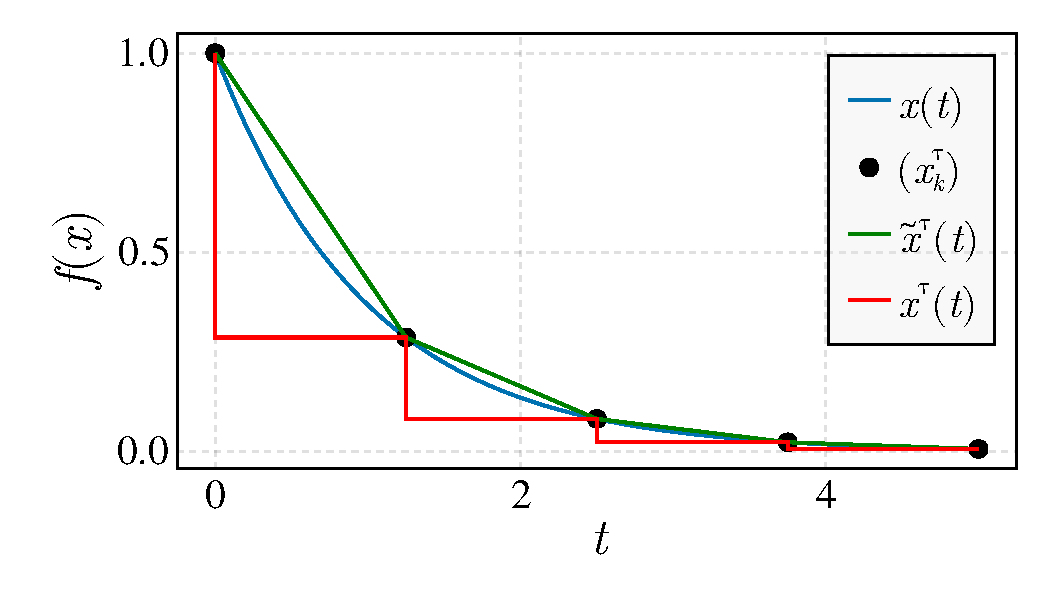
\includegraphics[width=0.6\textwidth]{../Notes-Portugues/Figures/eulerinterpolacao}
\end{center}
    \caption{Exemplo de aproximação da solução $x(t)$.}
    \label{fig:eulerinterpolacao}
\end{figure}

\end{frame}

\subsection{Fluxo de Gradiente em Wasserstein}
\begin{frame}[fragile]{Fluxo de Gradiente em Wasserstein}

	Queremos agora estender essa ideia do fluxo de gradiente
	para espaços os espaços de 2-Wasserstein, e vamos assumir também
	que nossas medidas de probabilidade são absolutamente contínuas em relação a Lebesgue.
	Vamos assim
	alterar nosso Esquema de Minimização de Movimento para
	\begin{equation}
		\rho_{k+1}^\tau \in \text{argmin}_{\rho} F(\rho)+\frac{W_2^2(\rho,\rho_k^\tau)}{2\tau},
		\label{EMMW}
	\end{equation}
	Onde $F$ agora não é mais uma função de $\mathbb R^n \to \mathbb R$, mas sim
	um funcional $F: \mathbb \mathcal P_2(\Omega) \to \mathbb R$, e.g.
	$F(\rho) = \int_\Omega f(\rho(x))dx$.

\end{frame}

\begin{frame}[fragile]{Fluxo de Gradiente em Wasserstein}

	\begin{equation}
		\rho_{k+1}^\tau \in \text{argmin}_{\rho} F(\rho)+\frac{W_2^2(\rho,\rho_k^\tau)}{2\tau}
	\end{equation}
	O problem de minimização acima é em um espaço de funções, onde buscamos a medida de
	probabilidade $\rho$ que minimiza. Assim, utilizaremos a ideia de \textbf{primeira variação}
	proveniente do Cálculo de Variações.

	Seja $G: \mathcal P(\Omega) \to \mathbb R$ um funcional, chamaremos
	$\frac{\delta G}{\delta \rho}(\rho)$ a primeira variação de $G$, caso
	exista uma função única (a menos de uma constante), tal que
	\begin{equation}
		\frac{d}{d\varepsilon} G(\rho + \varepsilon \chi)|_{\varepsilon =0} =
		\int \frac{\delta G}{\delta \rho}(\rho) d\chi,
	\end{equation}
	para toda perturbação $\chi$. Note a perturbação deve satisfazer $\int d\chi = 0$
	e além disso, deve existir pelo menos $\varepsilon \in [0,\varepsilon_0]$, tal
	que $\rho + \varepsilon \chi \in \mathcal P(\Omega)$.

\end{frame}

\begin{frame}[fragile]{Fluxo de Gradiente em Wasserstein}

	Análogamente ao caso em $\mathbb R$,
	se $\frac{\delta G}{\delta}(\rho^*) = 0$(ou constante), temos assim
	uma possível solução para o problema de otimização. Se provamos,
	por exemplo, que nosso funcional é contínuo
	em algum sentido, como em convergência fraca de probabilidade, e que
	é convexo. Teremos então existência e unicidade para esse problema de otimização,
	com $\rho^*$ sendo a função que minimiza.

\end{frame}

\begin{frame}[fragile]{Fluxo de Gradiente em Wasserstein}

	Se nosso funcional é $F(\rho)=\int_\Omega f(\rho(x))dx$, onde $f:\mathbb R \to \mathbb R$
	é convexa e superlinear, teremos que
	\begin{equation}
		\frac{\delta F}{\delta \rho}(\rho) = f'(\rho)
	\end{equation}.

	Além disso, podemos provar que para o funcional $\rho \mapsto W_2(\rho, \nu)$, temos que
	\begin{equation}
		\frac{\delta W_2(\cdot,\nu)}{\delta \rho}(\rho_0) = \phi.
	\end{equation}

\end{frame}

\begin{frame}[fragile]{Fluxo de Gradiente em Wasserstein}

	Lembrando que queremos minimiza a equação abaixo
	\begin{equation}
		\rho_{k+1}^\tau \in \text{argmin}_{\rho} F(\rho)+\frac{W_2^2(\rho,\rho_k^\tau)}{2\tau}.
	\end{equation}

	Temos então que no ponto de mínimo
	\begin{equation}
		\frac{\delta F}{\delta \rho}(\rho_{k+1}^\tau) + \frac{\phi}{\tau} = \text{const}.
	\end{equation}.

	Para $\mu\ll \lambda$, com $\Omega$ compacto, temos que nosso espaço 2-Wasserstein
	tem sempre um mapa $T(x) = x - \nabla \phi(x)$ (apresentamos na sessão de existência). Logo
	\begin{equation}
		-\bm{v}(x):= \frac{T(x)-x}{\tau} = -\frac{\phi(x)}{\tau} =
		\nabla (\frac{\delta F}{\delta \rho}(\rho))(x).
	\end{equation}
	Pela Equação de Benamou-Brenier, temos então que
	\begin{equation}
		\partial_t \rho - \nabla \cdot (\rho \nabla (\frac{\delta F}{\delta \rho}(\rho))(x) = 0.
	\end{equation}

\end{frame}

\begin{frame}[fragile]{Fluxo de Gradiente em Wasserstein}

	Finalmente, chegamos onde queríamos desde o começo.

	Se nosso funcional é $F(\rho)=\int_\Omega f(\rho(x))dx$, onde $f:\mathbb R \to \mathbb R$
	é convexa e superlinear, teremos que
	\begin{equation}
		\frac{\delta F}{\delta \rho}(\rho) = f'(\rho)
	\end{equation}.

	Mais ainda, se $f(t) = t \log t $ , temos que $f'(t) = 1+ \log t$ e que
	$\nabla(f'(\rho))=\frac{\nabla \rho}{\rho}$.

	E assim, chegamos na equação do calor:
	\begin{equation}
		\partial_t \rho - \nabla \cdot (\rho \nabla (\frac{\delta F}{\delta \rho}(\rho))(x) =
	\partial_t \rho - \Delta \rho -0.
	\end{equation}


\end{frame}

\begin{frame}[allowframebreaks]{References}
	\nocite{*}

% \renewcommand{\bibsection}{\section{}}
  \renewcommand{\section}[2]{}%
\tiny{\bibliography{ref}}
\bibliographystyle{plainnat}
  % \bibliographystyle{plain}
  % \bibliographystyle{abbrv}
  % \bibliographystyle{apa}
\end{frame}


\end{document}